\subsection{Customer Acceptance}
Per la macrofase Customer Acceptance sono previste 2 fasi da una settimana ciascuna:
\begin{itemize}
    \item Validazione requisiti obbligatori dal 2022-09-12 al 2022-09-19
    \item Validazione requisiti desiderabili dal 2022-09-20 al 2022-09-26
\end{itemize}
\subsubsection{Validazione requisiti obbligatori}
\begin{itemize}
    \item \textbf{Implementazione di test:} principalmente test di sistema;
    \item \textbf{Validazione e collaudo:} dei requisiti obbligatori;
    \item \textbf{Opzionale:} implementazione funzionalità creazione riunione;
    \item \textbf{Checkpoint:} per la descrizione dettagliata si veda \$4.1.2
\end{itemize}
\subsubsection{Validazione requisiti desiderabili}
\begin{itemize}
    \item \textbf{Validazione e collaudo:} dei requisiti facoltativi;
    \item \textbf{Approvazione:} il responsabile controlla, approva quanto realizzato in questa macrofase;
    \item \textbf{Checkpoint:} per la descrizione dettagliata si veda \$4.1.2
    \item \textbf{Presentazione CA:} viene effettuato il release del prodotto e di tutti i documenti. Viene preparata la presentazione per il colloquio finale.
\end{itemize}
\begin{figure}[H]
	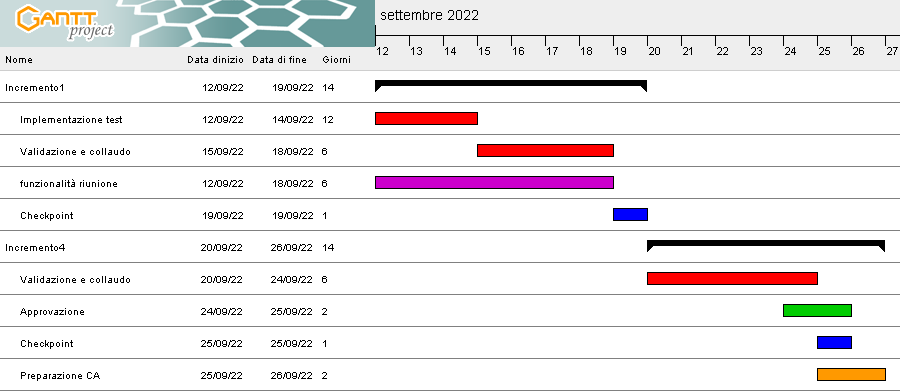
\includegraphics[width=\linewidth]{images/CA.png}
    \caption{Diagramma di Gantt - Macrofase CA}
\end{figure}
\newpage